\chapter{Диагоностика убегающих электронов на токамаке JET}
\label{ch:ch5}

% ==========================================================

\section{Спектрометы жёсткого рентгеновского излучения на токамаке JET}

В настоящее JET имеет самую совершенную систему гамма-спектрометрии среди действующих токамаков~\cite{Iliasova2022}. В экспериментах используются два спектрометра LaBr3(Ce) $\varnothing 76,2 \times 152,4$~мм~\cite{Nocente2010} с вертикальным и тангенциальным линиями обзора (рисунок~\ref{fig:jetHxrDetectorsScheme}, слева). Детектор с вертикальной линией обзора LaBr3(Ce) может быть заменён на один из двух других спектрометров. Первый --- HPGe-спектрометр~\cite{Tardocchi2011}, обеспечивающий высокоэффективную регистрацию гамма-излучения с исключительно высоким энергетическим разрешением (2,4~кэВ на линии 1,333~МэВ), который, однако, имеет гораздо меньшую по сравнению с LaBr3(Ce) максимальную скорость счёта. Второй --- спектрометр NaI(Tl) размером $\varnothing 5 \times 5$~дюймов, разрешение которого составляет 3\% на линии 4~МэВ~\cite{Tardocchi2008}. Спектрометр BGO с квазитангенциальной линией обзора, ранее работавший на токамаке, был заменен детектором LaBr3(Ce) ($\varnothing 76,2 \times 152,4$~мм)~\cite{Nocente2021}. В тангенциальном спектрометре полиэтиленовый аттенюатор был заменен на аттенюатор из гидрида лития (LiH)~\cite{Curuia2017}. На коллиматор вертикального спектрометра LaBr3(Ce) в дополнение к ранее существовавшему LiH-фильтру $\varnothing 30 \times 300$~мм, обогащенному изотопом ${}^6$Li, был установлен аттенюатор LiH с естественным соотношением изотопов лития длиной 400~мм~\cite{Murari2008}.

\begin{figure}[ht!]
  \centerfloat{ 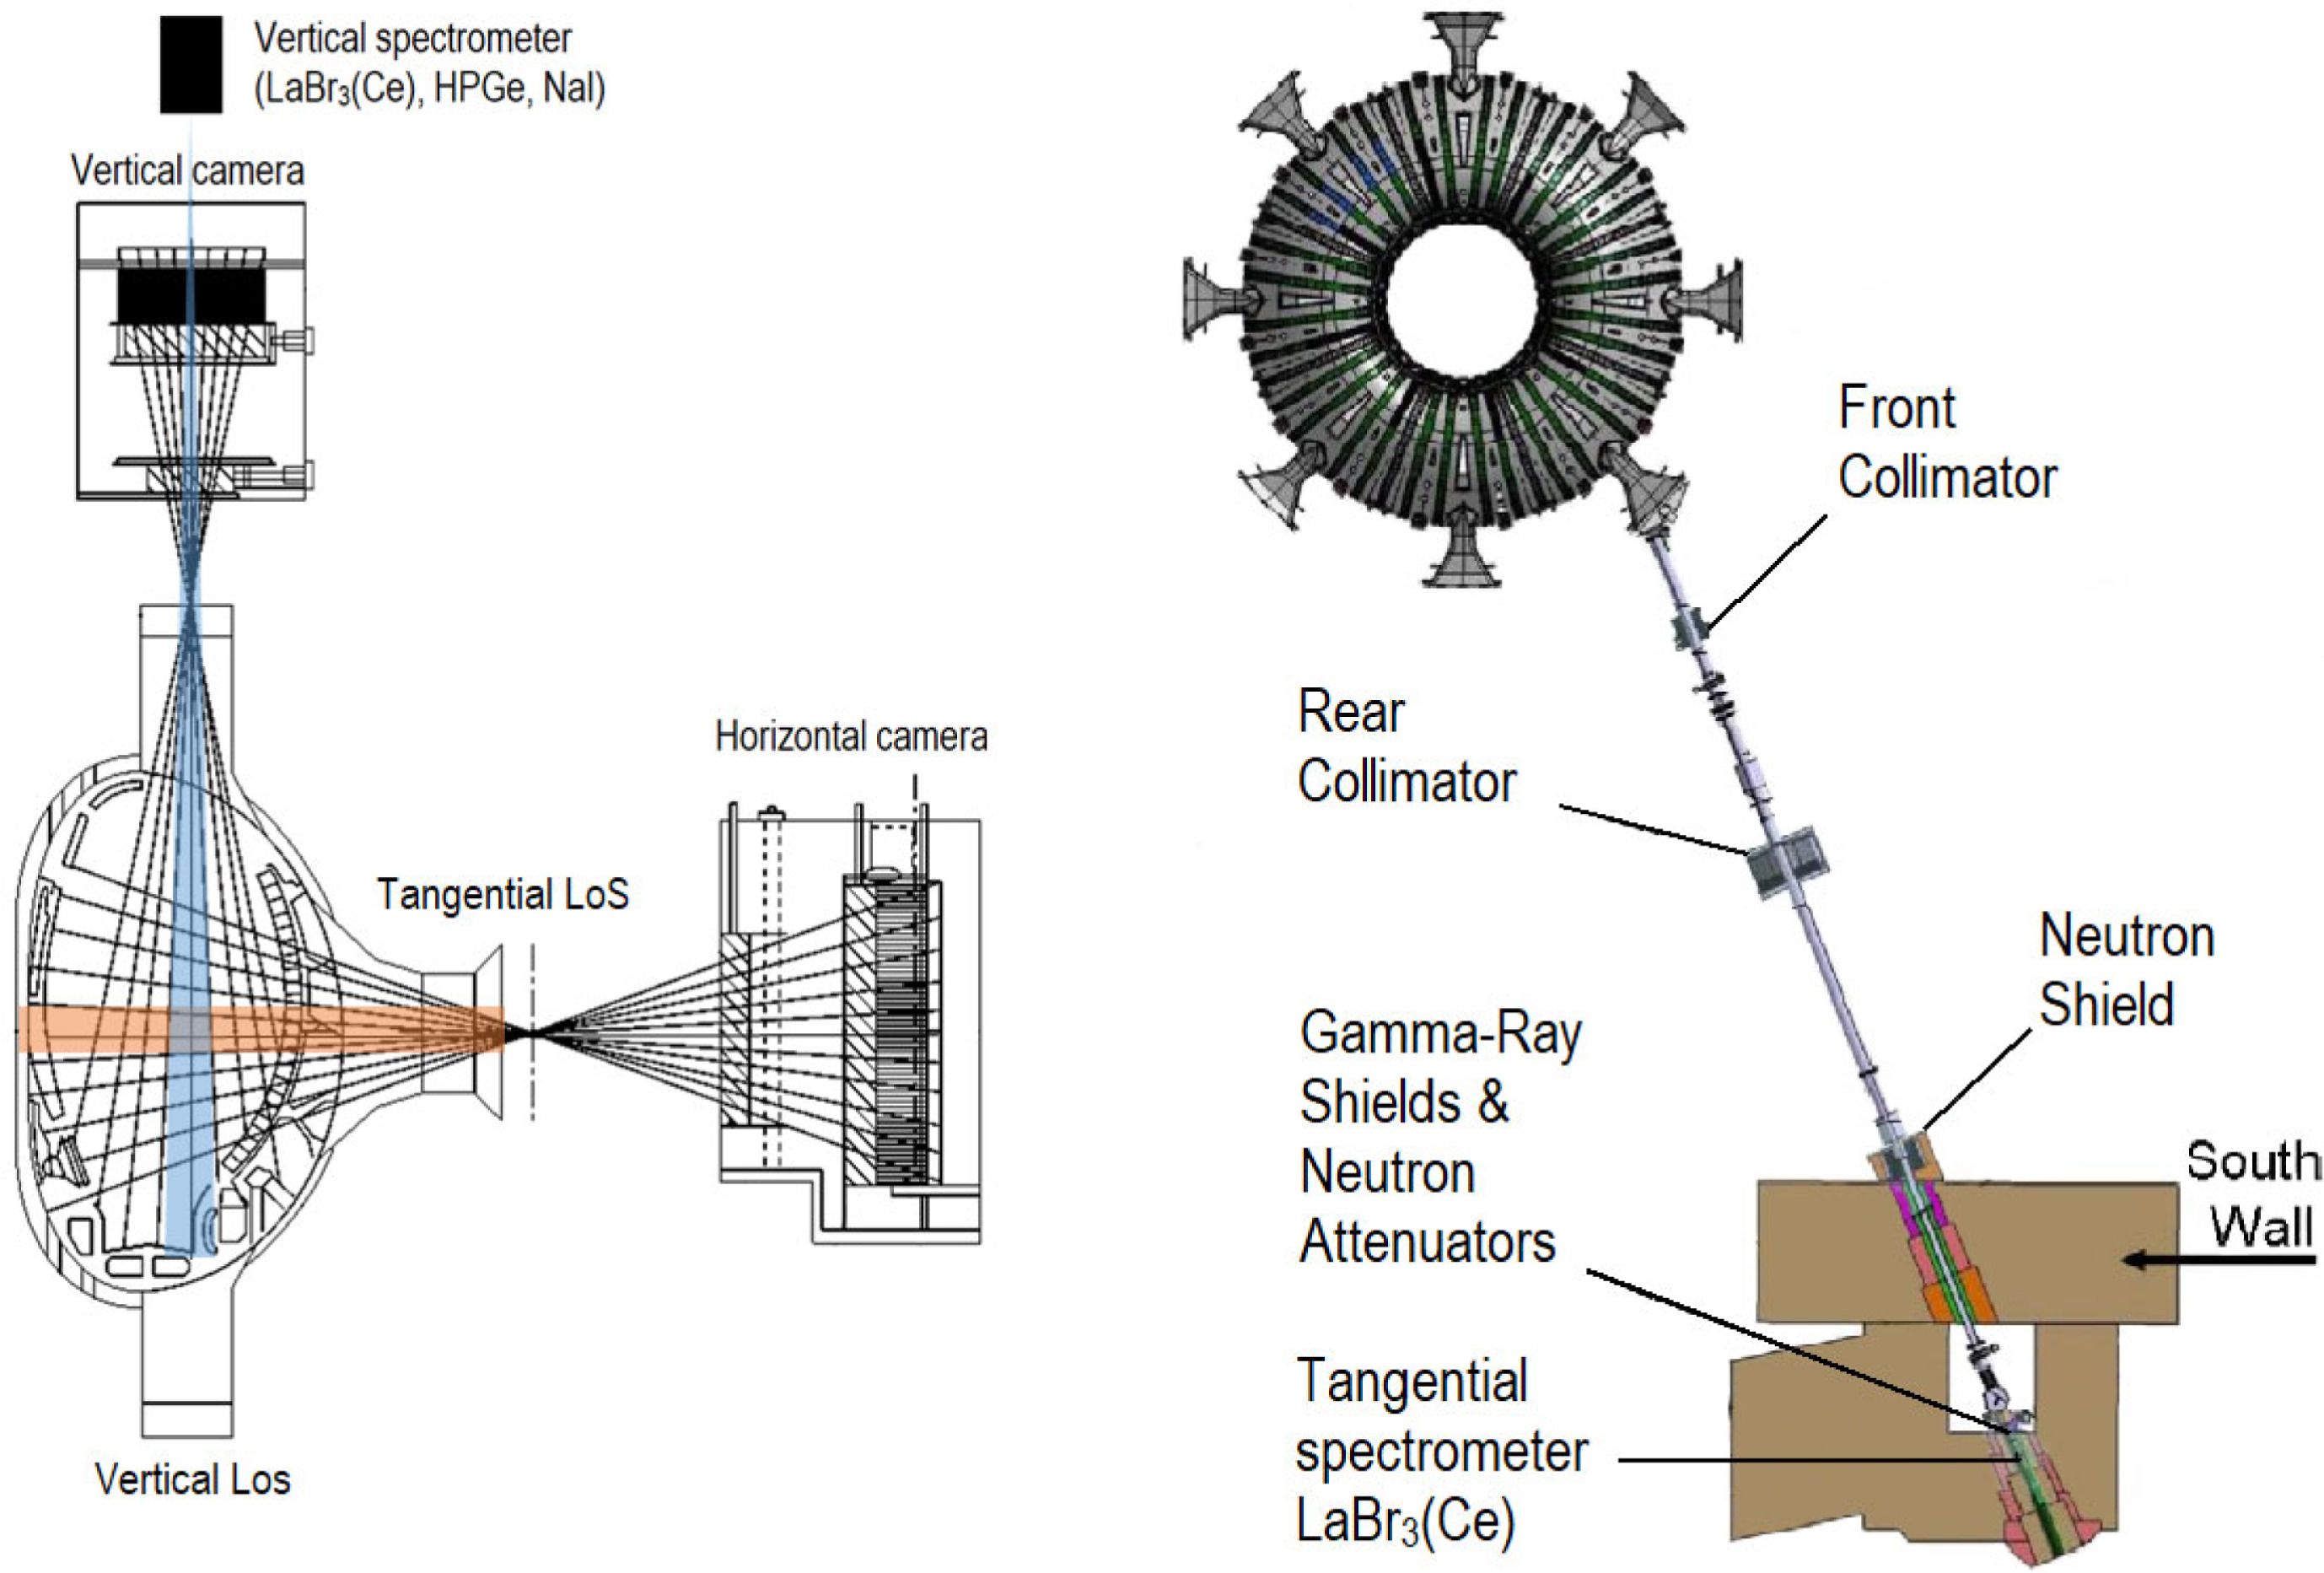
\includegraphics[width=0.92\linewidth]{jetHxrDetectorsScheme} }
  \caption{ Расположение гамма-спектрометров на токамаке JET.~\cite{Iliasova2022} }
  \label{fig:jetHxrDetectorsScheme}
\end{figure}

Сигнал со спектрометров LaBr3(Ce) записывается в сегментной моде~\cite{Pereira2008,Pereira2011} когда сохраняются только части осциллограммы, превышающие некоторый заданный порог, и их окрестности. Для оцифровки используется 14-битное АЦП с частотой 400~МГц. Сохранённые осциллограммы записываются в систему сбора и обработки данных CODAS, откуда могут быть впоследствии извлечены и обработаны, например, с помощью алгоритмов, описанных в главах~\ref{ch:ch2} и \ref{ch:ch3}. 

В дополнение к этим спектрометрам для получения двумерных измерений профилей гамма-излучения может использоваться гамма-камера, состоящая из 19~компактных детекторов с 10~горизонтальными и 9~вертикальными линиями обзора (рисунок~\ref{fig:jetHxrDetectorsScheme}, справа). Компактные детекторы изготовлены из кристаллов LaBr3(Ce) $\varnothing 25 \times 17$~мм~\cite{Rigamonti2018}. Выходной сигнал от каждого детектора оцифровывается 13-битном АЦП со скоростью 200 отсчётов в секунду~\cite{Fernandes2018}.

Все диагностики токамака JET сохраняют результаты измерений в системе CODAS~\cite{Jones1986}. Для обработки данных в компьютерный код ``DeGaSum'' была добавлена возможность загрузки данных из системы CODAS с всех вышеперечисленных гамма-диагностик. Для детекторов на основе BGO и HPGe доступны спектры, созданные в результате обработки с помощью программно-аппаратных средств диагностик. Для детекторов NaI(Tl), LaBr3(Ce) доступны осциллограммы, обработка которых с помощью продвинутых алгоритмов, описанных в главе~\ref{ch:ch2}, может позволить получить больше полезной информации. Итоговые спектры жёсткого рентгеновского излучения могут быть обработаны с помощью алгоритмов, описанных в главе~\ref{ch:ch3}. 

% ==========================================================

\section{Восстановление функции распределения убегающих электронов на токамаке JET}

Для восстановления функций распределения были предварительно рассчитаны функции отклика детектора и функции генерации убегающими электронами жёсткого рентгеновского излучения. Расчёты были выполнены А.~Е.~Шевелевым с помощью кода MCNP, примеры полученных функций показаны на рисунке~\ref{fig:jetGenerationFunctions}. 

\begin{figure}[ht!]
  \centerfloat{ 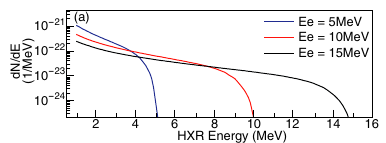
\includegraphics[width=0.85\linewidth]{jetGenerationFunctions} }
  \caption{ Спектры жёсткого рентгеновского излучения, генерируемые пучком моноэнергетических электронов с различной энергией, рассчитанные для условий токамака JET.~\cite{Shevelev2013} }
  \label{fig:jetGenerationFunctions}
\end{figure}


Разработанный код DeGaSum был использован для восстановления распределений убегающих электронов по измеренным спектрам жёсткого рентгеновского излучения на токамаке JET. Рисунок~\ref{fig:jetRunawayEdf82715} иллюстрируют применение кода DeGaSum для диагностики убегающих электронов на токамаке JET. В качестве примера можно рассмотреть разряд №~82715, в котором при нарастании тока возник пучок убегающих электронов. Спектры жёсткого рентгеновского излучения были измерены с помощью   детектором NaI(Tl) с вертикальной линией обзора, после чего были обработаны с помощью программы DeGaSum. Спектры излучения, генерируемые быстрыми электронами при взаимодействии с ионами плазмы и зарегистрированные спектрометром, показаны на верхних рисунках \ref{fig:jetRunawayEdf82715} черными точками. Восстановленные функции распределения убегающих электронов представлены красными линиями на нижних рисунках. Результаты свёрток полученных функций распределения с функциями отклика детектора показаны на рисунках синими линиями. В этом разряде генерация пучка убегающих электронов происходила при нарастании тока при малой плотности и прекращалась при увеличении плотности.~\cite{Shevelev2013} 

%\begin{figure}[ht!]
%  \centerfloat{ 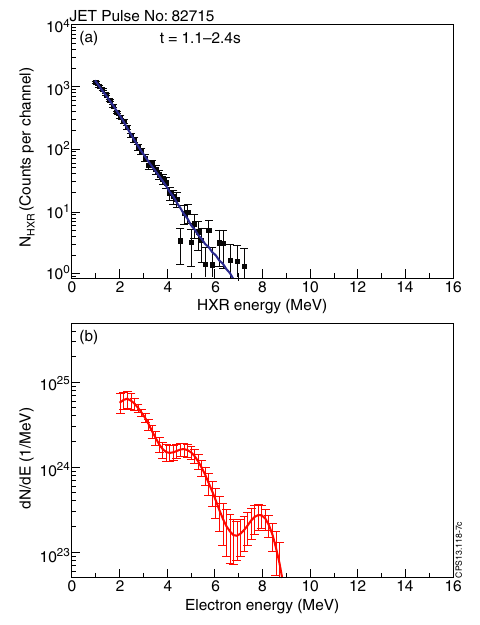
\includegraphics[width=0.55\linewidth]{jetRunawayEdf82715_t1} }
%  \caption{ (a) --- спектр жёсткого рентгеновского излучения, зарегистрированный в период 41,1--42,4 с помощью детектора NaI(Tl) в импульсе на токамаке JET №~82715 (черные точки), и спектр, полученный после свёртки восстановленной функции распределения электронов с функцией отклика детектора (синяя линия); (b) --- восстановленная функция распределения энергии убегающих электронов.~\cite{Shevelev2013} }
%  \label{fig:jetRunawayEdf82715_t1}
%\end{figure}
%
%\begin{figure}[ht!]
%  \centerfloat{ 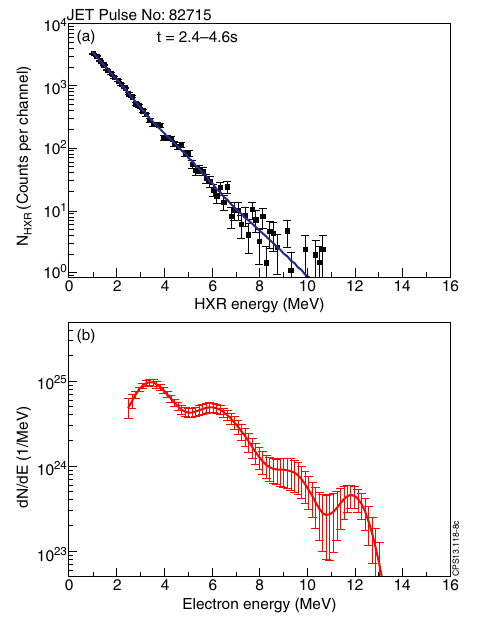
\includegraphics[width=0.55\linewidth]{jetRunawayEdf82715_t2} }
%  \caption{ (a) --- спектр жёсткого рентгеновского излучения, зарегистрированный в период 41,1--42,4 с помощью детектора NaI(Tl) в импульсе на токамаке JET №~82715 (черные точки), и спектр, полученный после свёртки восстановленной функции распределения электронов с функцией отклика детектора (синяя линия); (b) --- восстановленная функция распределения энергии убегающих электронов.~\cite{Shevelev2013} }
%  \label{fig:jetRunawayEdf82715_t2}
%\end{figure}
%
%\begin{figure}[ht!]
%  \centerfloat{ 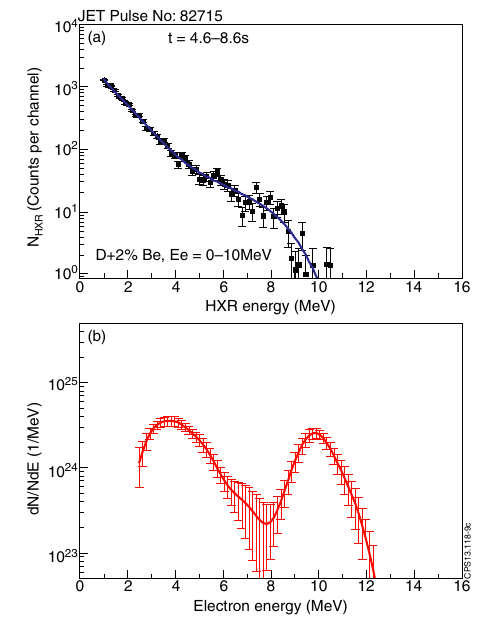
\includegraphics[width=0.55\linewidth]{jetRunawayEdf82715_t3} }
%  \caption{ (a) --- спектр жёсткого рентгеновского излучения, зарегистрированный в период 41,1--42,4 с помощью детектора NaI(Tl) в импульсе на токамаке JET №~82715 (черные точки), и спектр, полученный после свёртки восстановленной функции распределения электронов с функцией отклика детектора (синяя линия); (b) --- восстановленная функция распределения энергии убегающих электронов.~\cite{Shevelev2013} }
%  \label{fig:jetRunawayEdf82715_t3}
%\end{figure}

\begin{figure}[ht]
    \begin{minipage}[b][][b]{0.42\linewidth}\centering
        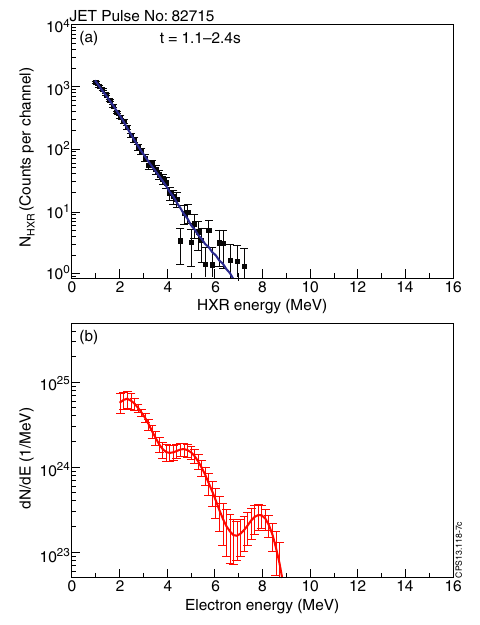
\includegraphics[width=0.98\linewidth]{jetRunawayEdf82715_t1} \\ а)
    \end{minipage}
    \hfill
    \begin{minipage}[b][][b]{0.42\linewidth}\centering
        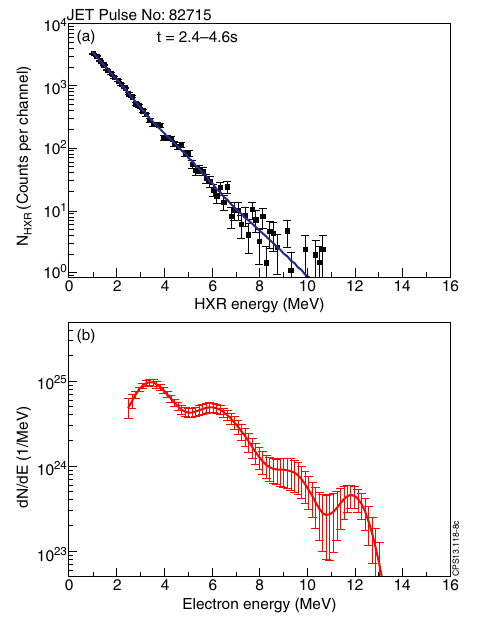
\includegraphics[width=0.98\linewidth]{jetRunawayEdf82715_t2} \\ б)
    \end{minipage}
    \hfill
    \begin{minipage}[b][][b]{0.42\linewidth}\centering
        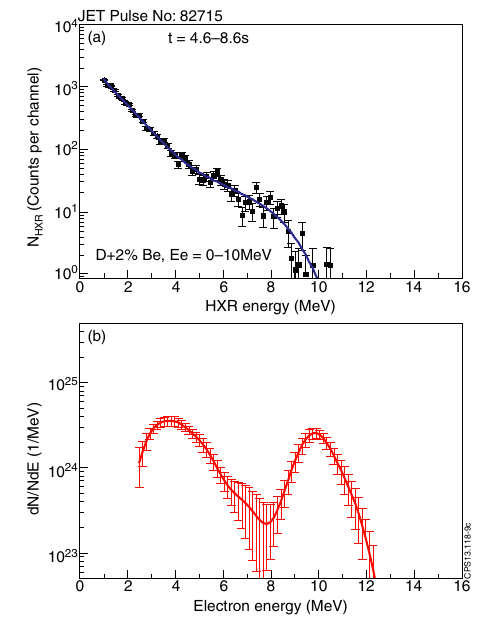
\includegraphics[width=0.98\linewidth]{jetRunawayEdf82715_t3} \\ в)
    \end{minipage}
    \caption{ Разряд на токамаке JET №~82715, результаты обработки данных с детектора NaI(Tl). Верхние изображения, чёрные точки --- зарегистрированный спектр жёсткого рентгеновского излучения, нижние изображения, красная кривая --- восстановленная функция распределения убегающих электронов, верхние изображения, синяя кривая --- спектр излучения, полученный в результате свёртки восстановленной функции распределения. (а) --- временное окно 41,1--42,4~с, (б) --- временное окно 42.4--44.6~с, (в) --- временное окно 44.6--48.6~с.~\cite{Shevelev2013}. }
    \label{fig:jetRunawayEdf82715}
\end{figure}



Мы не ставили целью теоретическое объяснение полученных результатов наших измерений. Разработанная методика позволяет анализировать процессы генерации и эволюции убегающего пучка и проводить верификацию теоретических моделей. Полученная нами в рассматриваемом разряде форма распределения может быть связана с тем, что детектор имеет коллимированную вертикальную линию обзора и может регистрировать излучение только из центральной части плазменного шнура.~\cite{Shevelev2013} Убегающий пучок может иметь пространственное распределение, зависящее от энергии. Это может быть возможно из-за эффекта смещения орбиты релятивистского убегающего пучка~\cite{Knoepfel1979}. Также форма распределения электронов может отражать эволюцию процесса убегающей генерации, включая режимы первичной и вторичной генерации~\cite{Helander2002}.

Ток убегания, создаваемый электронами с энергией более 2~МэВ, был определён путем интегрирования потока электронов, пересекающего вертикальное поле зрения спектрометра. Зависимость тока убегающих электронов от времени показана на рисунке~\ref{fig:jetPulseParams82715}~(d). Значения тока плазмы и усредненной по линии плотности электронов представлены на рисунках~\ref{fig:jetPulseParams82715}~(a) и (b) соответственно. Кривая скорости счета гамма-спектрометра NaI(Tl) показана на рисунке~\ref{fig:jetPulseParams82715}~(c). На рисунке~\ref{fig:jetPulseTomography82715} представлена томографическая реконструкция интенсивности излучения в камере токамака, полученная с помощью гамма-камеры.


\begin{figure}[ht]
    \begin{minipage}[b][][b]{0.48\linewidth}\centering
        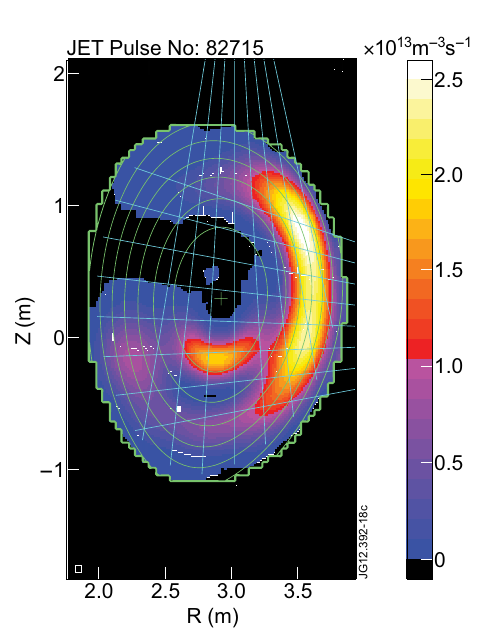
\includegraphics[width=0.95\linewidth]{jetPulseTomography82715_t1} \\ а)
    \end{minipage}
    \hfill
    \begin{minipage}[b][][b]{0.48\linewidth}\centering
        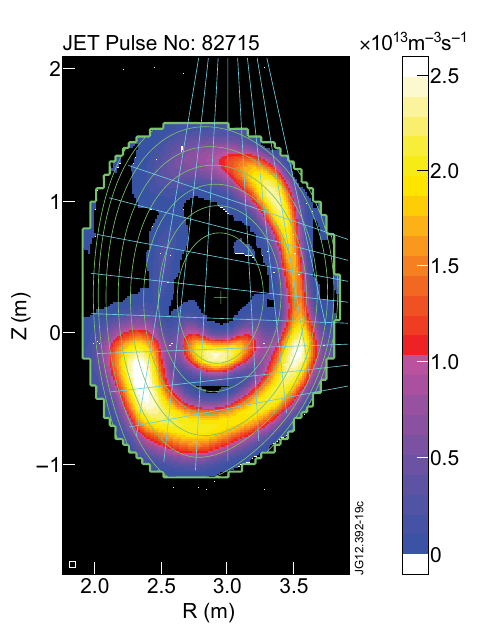
\includegraphics[width=0.95\linewidth]{jetPulseTomography82715_t2} \\ б)
    \end{minipage}
    \caption{ Томографическая реконструкция пространственного распределения жёсткого рентгеновского излучения в камере токамака JET в ходе разряда №~82715: (а) --- во временном интервале 41.1--41.8~c, (б) --- во временном интервале 42.4--43.4~с.~\cite{Shevelev2013a}. }
    \label{fig:jetPulseTomography82715}
\end{figure}

\begin{figure}[ht!]
  \centerfloat{ 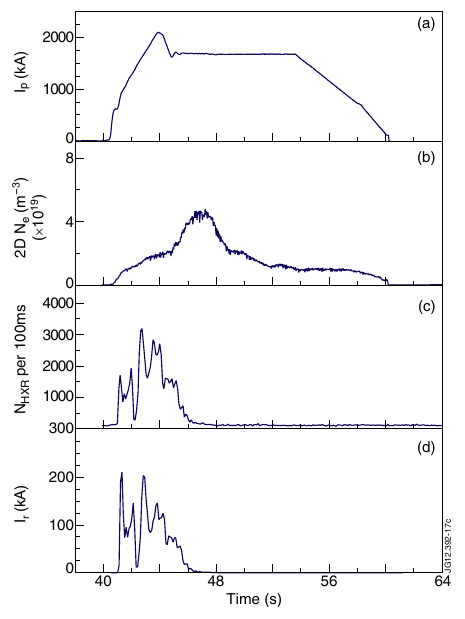
\includegraphics[width=0.75\linewidth]{jetPulseParams82715} }
  \caption{ (a) --- ток по плазме в разряде №~82715 на токамаке JET ($I_p = 1,7$~МА, $B_t = 2$~Тл, $T_e = 1,8$~кэВ, $P_{NBI} = 2,3$~МВт); (b) ---  плотность электронов; (c) интенсивность жёсткого рентгеновского излучнения; (d) --- восстановленный ток убегающих электронов в видимом для вертикального спектрометра объеме плазмы, учтены только электроны с энергией больше чем 2~МэВ.~\cite{Shevelev2013} }
  \label{fig:jetPulseParams82715}
\end{figure}


% ==========================================================

\FloatBarrier
\section{Убегающие электроны в экспериментах с ILW на токамаке JET}

Функция распределения убегающих электронов по энергии является важной характеристикой, описывающей процесс их генерации.~\cite{Plyusnin2015} Эволюция функции распределения может характеризовать различные стадии этого процесса, такие как ускорение электронов и их рассеяние на фоновой плазме и нейтральных частицах, взаимодействие с первой стенкой и т.д. Иногда убегающие электроны регистрировались и на переходных стадиях пробоя разряда и нарастания тока плазмы в токамаке JET с ИТЭР-подобной стенкой (JET-ILW).~\cite{Plyusnin2015} Генерация убегающих электронов во время стадии плато в ходе разрядов на токамаке JET представляют собой предмет повышенного интереса, в первую очередь из-за редкой возможности изучения возникновения, роста и причин гибели релятивистских электронов.~\cite{Granetz2014} 

Ниже в этом разделе представлены результаты исследования параметров убегающих элекронов, генерируемых и регистрируемых во время квазистационарной стадии разряда JET-ILW после значительного снижения плотности плазмы. Эволюция измеряемых параметров плазмы (плотность, температура электронов, напряжение контура, ток плазмы) была численно обработана в рамках традиционной теории генерации убегающих электронов.~\cite{Plyusnin2015}

Во время стадии плато обычного разряда JET-ILW №~86078 внезапная потеря контроля над впуском рабочего газа привела к снижению плотности плазмы до чрезвычайно низкого значения: $ < n_e > \le 2.0\cdot10^{18}$~м${}^{-3}$, начиная с отметки времени примерно $t = 18.4$~с на рисунке~\ref{fig:jetPulseParams86078}. Этот режим с низкой плотностью сохраняется в течении приблизительно 8~секунд. Нейтронная диагностика зафиксировала практически полное исчезновение выхода термоядерных нейтронов из дейтериевой плазмы после этого уменьшения плотности. Плазменный ток во время этой стадии низкой плотности поддерживался почти постоянным ($I_{pl} \approx 1.8$~МА) до прекращения разряда. Измеренное напряжение обхода $V_{loop}$ в начале фазы снижения плотности составило $V_{loop} = 0.65$~В, что соответствует $<T_e> = 1,5$~кэВ, если проводить вычисление по классическому сопротивлению с неоклассической поправкой на долю захваченных частиц.~\cite{Plyusnin2015} Полученное значение $<T_e>$ очень близко к величине $T_e$, предоставляемым другими диагностиками JET. В фазе низкой плотности средняя дрейфовая скорость увеличивается до $u_0 = (I_{pl}/\pi a_{pl}^2 )/(e n_e) \le 3,0\cdot10^6$~м/с, где $a_{pl}$ --- радиус плазменного шнура, полученный с помощью EFIT, а $<n_e>$ --- измеренная плотность плазмы. Большая дрейфовая скорость $u_0 \approx 0.1 \times v_{Te}$ ведёт к асимметрии функции распределения электронов 
\begin{equation*}
  f_e(v_e) \sim n_e \times \exp \left( -\frac{ ( v_e - u_0 )^2 }{ v_{te}^2 } \right)
\end{equation*}
Расчет показывает, что возникшая асимметрия вызывает значительное увеличение числа электронов (до примерно 10\%), движущихся в направлении ускорения. Это приводит к увеличению числа электронов со скоростями выше критической (выражение~\ref{eq:critVelocity}).

\begin{figure}[ht!]
  \centerfloat{ 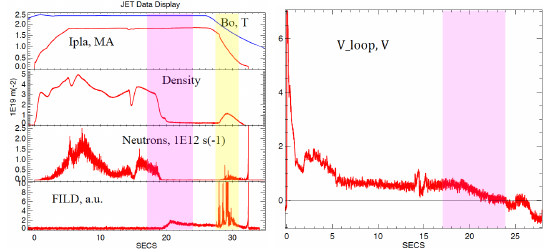
\includegraphics[width=0.85\linewidth]{jetPulseParams86078} }
  \caption{ Разряд №~86078 на токамаке JET. Слева --- эволюция различных параметров разряда, справа --- измерение напряжения обхода от времени. На обоих графиках розовым  выделена исследуемая стадия эволюции убегающих электронов, желтым --- фаза нестабильности пучка убегающих электронов.~\cite{Plyusnin2015} }
  \label{fig:jetPulseParams86078}
\end{figure}

Согласно теории генерации убегающих электронов, за генерацию ответственны два механизма: первичный механизм, когда ускорение электронов внешним электрическим полем превышает сопротивление трения кулоновских столкновений с частицами плазмы, и вторичная лавина, когда существующие убегающие электроны передают часть энергии окружающим тепловым электронам за счет близких столкновений, что переводит их в режим убегания и позволяет увеличивать количество убегающих электронов в плазме. Ясно, что вторичное лавинообразование может произойти только в том случае, если первичная генерация обеспечит существенный поток убегающих электронов с достаточной энергией. 
%Заметим, что столкновения на близком расстоянии в 8*lnΛ менее часты, чем обычные кулоновские (дальние) столкновения. 
Динамика обоих процессов определяется в основном отношениями приложенного электрического поля к полю Дрейсера для процесса первичной генерации $\alpha = E_0/E_{D}$ (формула~\ref{eq:dreicerField}) и к критическом полю для лавинного механизма $\beta = E_0 / E_c $ (формула~\ref{eq:criticalField}).

\begin{figure}[ht!]
  \centerfloat{ 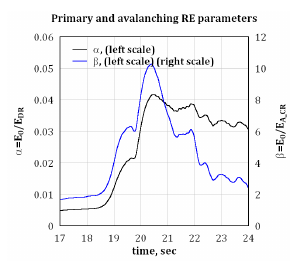
\includegraphics[width=0.85\linewidth]{jetPulseAlphaBeta86078} }
  \caption{ Разряд №~86078 на токамаке JET. Эволюция параметров $\alpha$ и $\beta$ от времени.~\cite{Plyusnin2015} }
  \label{fig:jetPulseAlphaBeta86078}
\end{figure}

На рисунке~\ref{fig:jetPulseAlphaBeta86078} представлена эволюция параметров $\alpha$ и $\beta$ на стадии низкой плотности. Генерация убегающих электронов моделировалась с помощью уравнений эволюции плотности
\begin{equation*}
  \frac{ d n_{RE} }{ d t } = \lambda_R - \frac{ n_{RE} }{ \tau_R } + \frac{ n_{RE} }{ t_0 }
\end{equation*}
где $\lambda_R$ --- скорость генерации первичных электронов, а параметр $t_0 \sim 1/(\beta - 1 )$ отвечает за генерацию вторичных электронов, $\tau_R$ --- время удержания убегающих электронов, которое далее предполагалось бесконечно большим.

Моделирование выявило значительное увеличение скорости образования и одновременное снижение критической энергии убегания $\varepsilon_c = v_c^2 m_e /2$ (формула~\ref{eq:critVelocity}) при снижении плотности ниже $10^{19}$~м${}^{-3}$, т.е. при $t \ge 19.5$~с (рисунок~\ref{fig:jetPulseCriticalEnergy86078}). Важно отметить, что вклад от лавинного механизма генерации в общую популяцию убегающих электронов меньше, чем ожидалось; основной механизм --- это дрейсеровское ускорение при асимметричной функции распределения по энергии ($n_{RE} \approx 10^{15}$~м${}^{-3}$ при $t = 24$~с), что соответствует току убегающих электронов $I_{RE} \le 200$~кА/м${}^2$. Эволюция функции распределения убегающих электронов свидетельствует о том, что дальнейшее поддержание тока убегающих электронов обеспечивается за счет лавинного маханизма. Постепенное уменьшение напряжения контура указывает не только на увеличение средней температуры $<T_e>$, но и на увеличение доли убегающих электронов в общем токе плазмы $I_{pl} \approx 1.8$~МА. 
%Напряжение обхода становится отрицательным при большой доле тока убегающих электронов. 
После $t = 24$~с численный анализ экспериментальных данных невозможен из-за того, что напряжения контура инвертируется (меняет знак на противоположный). Одновременно с увеличением числа убегающих электронов вертикальный и горизонтальный детекторы жёсткого рентгеновского излучения регистрировали увеличение интенсивности излучения от центра плазмы (рисунок~\ref{fig:jetPulseHxrNaI86078}). Сцинтилляционный детектор FILD (Fast Ions Loss Diagnostics, рисунок~\ref{fig:jetPulseParams86078}) также зарегистрировал усиление сигнала, что связано с наличием жёсткого рентгеновского излучения, сгенерированного убегающими электронами. На рисунке~\ref{fig:jetPulseHxrTomography86078} представлена томографическая реконструкция профиля рентгеновского излучения из плазмы, выполненная на основе данных с гамма-камеры токамака JET.

Спектрометрия так же использовалась для изучения динамики процесса генерации убегающих электронов (рисунок~\ref{fig:jetPulseEdf86078}). Были восстановлены распределения убегающих электронов по энергии, максимальная энергия убегающих электронов составила 7~МэВ, характерная энергия --- 2.5~МэВ.

\begin{figure}[ht!]
  \centerfloat{ 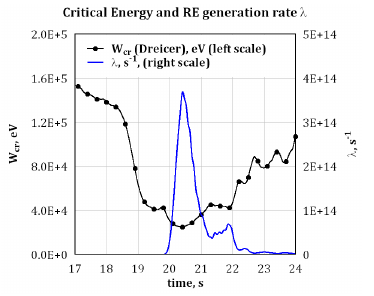
\includegraphics[width=0.65\linewidth]{jetPulseCriticalEnergy86078} }
  \caption{ Разряд №~86078 на токамаке JET. Эволюция критической энергии (ось слева, чёрные точки) и скорости генерации (ось справа, синяя кривая) от времени.~\cite{Plyusnin2015} }
  \label{fig:jetPulseCriticalEnergy86078}
\end{figure}

\begin{figure}[ht!]
  \centerfloat{ 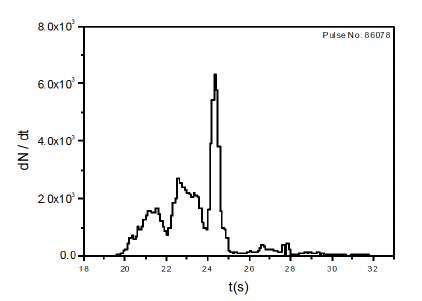
\includegraphics[width=0.65\linewidth]{jetPulseHxrNaI86078} }
  \caption{ Разряд №~86078 на токамаке JET. Скорость счёта детектора жёсткого рентгеновского излучения NaI(Tl) с вертикальной линией обзора.~\cite{Plyusnin2015} }
  \label{fig:jetPulseHxrNaI86078}
\end{figure}

\begin{figure}[ht!]
  \centerfloat{ 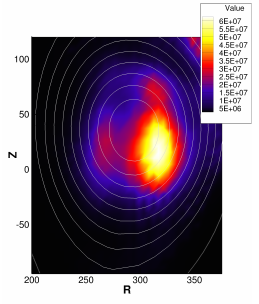
\includegraphics[width=0.55\linewidth]{jetPulseHxrTomography86078} }
  \caption{ Разряд №~86078 на токамаке JET. Томографическая реконструкция эмиссии жёсткого рентгеновского излучения по данным с гамма-камеры.~\cite{Plyusnin2015} }
  \label{fig:jetPulseHxrTomography86078}
\end{figure}

\begin{figure}[ht!]
  \centerfloat{ 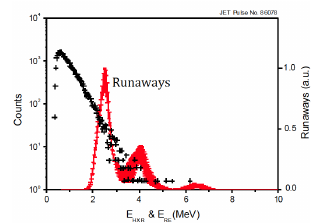
\includegraphics[width=0.65\linewidth]{jetPulseEdf86078} }
  \caption{ Разряд №~86078 на токамаке JET. Измеренный спектр жёсткого рентгеновского излучения (чёрные точки) и восстановленная функция распределения убегающих электронов (временное окно с 20.2 до 22.0~с).~\cite{Plyusnin2015} }
  \label{fig:jetPulseEdf86078}
\end{figure}

% ==========================================================

\FloatBarrier
\section{Выводы к главе 5}

На токамаке JET работают в настоящее время и работали в прошлом множество диагностик жёсткого рентгеновского излучения на основе сцинтилляционных кристаллов NaI(Tl), BGO, LaBr3(Ce), а так же полупроводниковый детектор HPGe высокого разрешения. Отдельно стоит упомянуть гамма-камеру, с помощью которой возможно выполнять томографическую реконструкцию двумерного профиля источника рентгеновского излучения в плазме. Результаты измерения записываются в систему хранения данных CODAS, из которой они впоследствии могут быть извлечены и обработаны. 

С помощью компьютерного кода ``DeGaSum'' была проведена обработка результатов измерений жёсткого рентгеновского излучения, сгенерированного убегающими электронами в плазме. Для этого с помощью компьютерного кода MCNP были рассчитаны аппаратные функции детекторов BGO и NaI(Tl), а так же функции генерации убегающими электронами жёсткого рентгеновского излучения. Затем была отработана процедура восстановления функции распределения убегающих электронов по энергии. Возможно восстановление функции распределения в выбранном временном окне, таким образом возможно отследить эволюцию функции распределения во времени. Приведены результаты такого восстановления для нескольких разрядов. 

Были рассмотрены и обработаны результаты измерения жёсткого рентгеновского излучения в разряде №~86078 на токамаке JET. В этом разряде внезапная потеря контроля над впуском рабочего газа привела к снижению плотности плазмы. Было исследовано поведение пучка убегающих электронов во время данного разряда, определены функция распределения и максимальная энергия убегающих электронов. 

% ==========================================================

\clearpage
